\begin{testproblem}
\begin{equation}
\min_{x\in\R^2}\ \tfrac{1}{2} x^T Q x + q^T x + c
\end{equation}
\begin{equation*}
\begin{split}
-10 \leq x_i & \leq 10,\quad i = 1,2 \\
\end{split}
\end{equation*}
\end{testproblem}

\begin{testproblem}
\begin{equation}
\min_{x\in\R^2}\ \| x-x_d \|^2 
\end{equation}
\begin{equation*}
\begin{split}
-10 \leq x_i & \leq 10,\quad i = 1,2 \\
\end{split}
\end{equation*}
\end{testproblem}

\begin{testproblem}
\begin{equation}
\min_{x\in\R^3}\ e^{\|x\|^2} 
\end{equation}
\begin{equation*}
\begin{split}
-10 \leq x_i & \leq 10,\quad i = 1,2,3 \\
\end{split}
\end{equation*}
\end{testproblem}

\begin{testproblem}
Rosenbrock-Funktion (vgl. Beispiel 1.4.1 in \cite[S.~14]{alt})
\begin{equation}
\min_{x\in\R^2}\ 100 (x_2-x_1^2)^2+(1-x_1)^2 
\end{equation}
\begin{equation*}
\begin{split}
-10 \leq x_i & \leq 10,\quad i = 1,2 \\
\end{split}
\end{equation*}
\end{testproblem}

\begin{testproblem}
Himmelblau-Funktion (vgl. Beispiel 1.4.2 in \cite[S.~14f]{alt})
\begin{equation}
\min_{x\in\R^2}\ (x_1^2+x_2-11)^2 + (x_1+x_2^2-7)^2 
\end{equation}
\begin{equation*}
\begin{split}
-10 \leq x_i & \leq 10,\quad i = 1,2 \\
\end{split}
\end{equation*}
\end{testproblem}

\begin{testproblem}
Bazaraa-Shetty-Funktion (vgl. Beispiel 1.4.3 in \cite[S.~15f]{alt})
\begin{equation}
\min_{x\in\R^2}\ (x_1-2)^4+(x_1-2 x_2)^2 
\end{equation}
\begin{equation*}
\begin{split}
-10 \leq x_i & \leq 10,\quad i = 1,2 \\
\end{split}
\end{equation*}
\end{testproblem}

\begin{testproblem}
(vgl. Beispiel 1.4.4 in \cite[S.~16]{alt})
\begin{equation}
\min_{x\in\R^2}\ (1.5-x_1 (1-x_2))^2+(2.25-x_1 (1-x_2^2))^2+(2.625-x_1 (1-x_2^3))^2 
\end{equation}
\begin{equation*}
\begin{split}
-10 \leq x_i & \leq 10,\quad i = 1,2 \\
\end{split}
\end{equation*}
\end{testproblem}

\begin{testproblem}
\begin{equation}
\min_{x\in\R^2}\ (1-x_1)^2+(x_1^2-x_2)^2+(1-x_2)^2 
\end{equation}
\begin{equation*}
\begin{split}
-10 \leq x_i & \leq 10,\quad i = 1,2 \\
\end{split}
\end{equation*}
\end{testproblem}

\begin{testproblem}
\begin{equation}
\min_{x\in\R^4}\ 100 (x_2-x_1^2)^2 + (1-x_1)^2 + 90 (x_4-x_3^2)^2 + (1-x_3)^2 + 10.1 ((x_2-1)^2 + (x_4-1)^2) + 19.8 (x_2-1) (x_4-1) 
\end{equation}
\begin{equation*}
\begin{split}
-10 \leq x_i & \leq 10,\quad i = 1,\ldots,4 \\
\end{split}
\end{equation*}
\end{testproblem}

\begin{testproblem}
\begin{equation}
\min_{x\in\R^2}\ \tfrac{1}{2} x^T Q x + q^T x + c
\end{equation}
\begin{equation*}
\begin{split}
-1 \leq x_1 & \leq 1 \\
-1 \leq x_2 & \leq 2 \\
\end{split}
\end{equation*}
\end{testproblem}

\begin{testproblem}
\begin{equation}
\min_{x\in\R^3}\ e^{\|x\|^2} 
\end{equation}
\begin{equation*}
\begin{split}
1 \leq x_1 & \leq 10 \\
0.5 \leq x_2 & \leq 10 \\
1 \leq x_3 & \leq 10 \\
\end{split}
\end{equation*}
\end{testproblem}

\begin{testproblem}
\begin{equation}
\min_{x\in\R^2}\ (x_1^2+x_2-11)^2 + (x_1+x_2^2-7)^2 
\end{equation}
\begin{equation*}
\begin{split}
5 \leq x_i & \leq 10,\quad i = 1,2 \\
\end{split}
\end{equation*}
\end{testproblem}

\begin{testproblem}
\begin{equation}
\min_{x\in\R^3}\ \| x-x_d \|^2 
\end{equation}
\begin{equation*}
\begin{split}
5 \leq x_i & \leq 10,\quad i = 1,2,3 \\
\end{split}
\end{equation*}
\end{testproblem}

\begin{testproblem}
\begin{equation}
\min_{x\in\R^2}\ (1-x_1)^2+(x_1^2-x_2)^2+(1-x_2)^2 
\end{equation}
\begin{equation*}
\begin{split}
-10 \leq x_1 & \leq 2 \\
-10 \leq x_2 & \leq -5 \\
\end{split}
\end{equation*}
\end{testproblem}

\begin{testproblem}
\begin{equation}
\min_{x\in\R^2}\ f(x) %TODO write f(x)
% y = 0;
% 	m = length(xi);
% 	for k=1:m
% 		y = y + ( x(1)*xi(k) + x(2) - eta(k) )^2;
% 	end
\end{equation}
\begin{equation*}
\begin{split}
-10 \leq x_i & \leq 10,\quad i = 1,2 \\
\end{split}
\end{equation*}
\end{testproblem}

\begin{testproblem}
\begin{equation}
\min_{x\in\R^3}\ f(x) %TODO write f(x)
% y = 0;
% 	m = length(xi);
% 	for k=1:m
% 		y = y + ( x(1)*(xi(k) - x(2))^2 + x(3) - eta(k) )^2;
% 	end
\end{equation}
\begin{equation*}
\begin{split}
-10 \leq x_i & \leq 20,\quad i = 1,2,3 \\
\end{split}
\end{equation*}
\end{testproblem}

\begin{testproblem}
\begin{equation}
\min_{x\in\R^2}\ f(x) %TODO write f(x)
% y = 0;
% 	for k=1:m
% 		y = y + ( x(1)*exp(xi(k)*x(2)) - eta(k) )^2;
% 	end
\end{equation}
\begin{equation*}
\begin{split}
-10 \leq x_i & \leq 10,\quad i = 1,2 \\
\end{split}
\end{equation*}
\end{testproblem}

\begin{testproblem}
(vgl. Beispiel 16.2 in \cite[S.~452]{nocedal}
\begin{equation}
\min_{x\in\R^3}\ \tfrac{1}{2} x^T Q x + q^T x + c
\end{equation}
\begin{equation*}
\begin{split}
x_1 + x_3 & = 3 \\
x_2 + x_3 & = 0 \\
\end{split}
\end{equation*}
\end{testproblem}

\begin{testproblem}
\begin{equation}
\min_{x\in\R^5}\ \| x-x_d \|^2 
\end{equation}
\begin{equation*}
\begin{split}
x_1 + x_2 + x_3 + x_4 + x_5 & = 1 \\
\end{split}
\end{equation*}
\end{testproblem}

\begin{testproblem}
(vgl. Problem 28 in \cite[S.~51]{hock})
\begin{equation}
\min_{x\in\R^3}\ \tfrac{1}{2} x^T Q x + q^T x + c
\end{equation}
\begin{equation*}
\begin{split}
x_1 + 2 x_2 + 3 x_3 & = 1 \\
\end{split}
\end{equation*}
\end{testproblem}

\begin{testproblem}
(vgl. Problem 48 in \cite[S.~71]{hock})
\begin{equation}
\min_{x\in\R^5}\ \tfrac{1}{2} x^T Q x + q^T x + c
\end{equation}
\begin{equation*}
\begin{split}
x_1 + x_2 + x_3 + x_4 + x_5 & = 5 \\
x_3 - 2 x_4 - 2 x_5 & = -3 \\
\end{split}
\end{equation*}
\end{testproblem}

\begin{testproblem}
(vgl. Problem 51 in \cite[S.~74]{hock})
\begin{equation}
\min_{x\in\R^5}\ \tfrac{1}{2} x^T Q x + q^T x + c
\end{equation}
\begin{equation*}
\begin{split}
x_1 + 3 x_2 & = 4 \\
x_3 + x_4 - 2 x_5 & = 0 \\
x_2 - x_5 & = 0 \\
\end{split}
\end{equation*}
\end{testproblem}

\begin{testproblem}
(vgl. Problem 52 in \cite[S.~75]{hock})
\begin{equation}
\min_{x\in\R^5}\ \tfrac{1}{2} x^T Q x + q^T x + c
\end{equation}
\begin{equation*}
\begin{split}
x_1 + 3 x_2 & = 0 \\
x_3 + x_4 - 2 x_5 & = 0 \\
x_2 - x_5 & = 0 \\
\end{split}
\end{equation*}
\end{testproblem}

\begin{testproblem}
(vgl. Problem 53 in \cite[S.~76]{hock})
\begin{equation}
\min_{x\in\R^5}\ \tfrac{1}{2} x^T Q x + q^T x + c
\end{equation}
\begin{equation*}
\begin{split}
x_1 + 3 x_2 & = 0 \\
x_3 + x_4 - 2 x_5 & = 0 \\
x_2 - x_5 & = 0 \\
-10 \leq x_i & \leq 10,\quad i = 1,\ldots,5 \\
\end{split}
\end{equation*}
\end{testproblem}

\begin{testproblem}
(vgl. Problem 49 in \cite[S.~72]{hock})
\begin{equation}
\min_{x\in\R^5}\ (x_1-x_2)^2 + (x_3-1)^2 + (x_4-1)^2 + (x_5-1)^6 
\end{equation}
\begin{equation*}
\begin{split}
x_1 + x_2 + x_3 + 4 x_4 & = 7 \\
x_3 + 5 x_5 & = 6 \\
\end{split}
\end{equation*}
\end{testproblem}

\begin{testproblem}
(vgl. Problem 50 in \cite[S.~73]{hock})
\begin{equation}
\min_{x\in\R^5}\ (x_1-x_2)^2 + (x_2-x_3)^2 + (x_3-x_4)^4 + (x_4-x_5)^2 
\end{equation}
\begin{equation*}
\begin{split}
x_1 + 2 x_2 + 3 x_3 & = 6 \\
x_2 + 2 x_3 + 3 x_4 & = 6 \\
x_3 + 2 x_4 + 3 x_5 & = 6 \\
\end{split}
\end{equation*}
\end{testproblem}

\begin{testproblem}
\begin{equation}
\min_{x\in\R^2}\ \tfrac{1}{2} x^T Q x + q^T x + c
\end{equation}
\begin{equation*}
\begin{split}
2 x_1 + x_2 & \leq 2 \\
x_1 - x_2 & \leq 1 \\
-x_1 - x_2 & \leq 1 \\
-2 x_1 + x_2 & \leq 2 \\
\end{split}
\end{equation*}
\end{testproblem}

\begin{testproblem}
(vgl. Beispiel 16.4 in \cite[S.~475]{nocedal})
\begin{equation}
\min_{x\in\R^2}\ \| x-x_d \|^2 
\end{equation}
\begin{equation*}
\begin{split}
-x_1 + 2 x_2 & \leq 2 \\
x_1 + 2 x_2 & \leq 6 \\
x_1 - 2 x_2 & \leq 2 \\
0 & \leq x_i,\quad i = 1,2 \\
\end{split}
\end{equation*}
\end{testproblem}

\begin{testproblem}
\begin{equation}
\min_{x\in\R^2}\ 100 (x_2-x_1^2)^2+(1-x_1)^2 
\end{equation}
\begin{equation*}
\begin{split}
-x_2 & \leq -1.5 \\
\end{split}
\end{equation*}
\end{testproblem}

\begin{testproblem}
(vgl. Beispiel 13.2 in \cite[S.~415f]{antoniou})
\begin{equation}
\min_{x\in\R^4}\ \tfrac{1}{2} x^T Q x + q^T x + c
\end{equation}
\begin{equation*}
\begin{split}
-x_1 & \leq 0 \\
-x_2 & \leq 0 \\
x_1 + 2 x_2 & \leq 2 \\
-x_4 & \leq -2 \\
-x_3 - x_4 & \leq -3 \\
x_3 + 2 x_4 & \leq 6 \\
\end{split}
\end{equation*}
\end{testproblem}

\begin{testproblem}
(vgl. Problem 21 in \cite[S.~44]{hock})
\begin{equation}
\min_{x\in\R^2}\ \tfrac{1}{2} x^T Q x + q^T x + c
\end{equation}
\begin{equation*}
\begin{split}
-10 x_1 + x_2 & \leq -10 \\
2 \leq x_1 & \leq 50 \\
-50 \leq x_2 & \leq 50 \\
\end{split}
\end{equation*}
\end{testproblem}

\begin{testproblem}
(vgl. Problem 35 in \cite[S.~58]{hock})
\begin{equation}
\min_{x\in\R^3}\ \tfrac{1}{2} x^T Q x + q^T x + c
\end{equation}
\begin{equation*}
\begin{split}
x_1 + x_2 + 2 x_3 & \leq 3 \\
0 & \leq x_i,\quad i = 1,2,3 \\
\end{split}
\end{equation*}
\end{testproblem}

\begin{testproblem}
(vgl. Problem 76 in \cite[S.~96]{hock})
\begin{equation}
\min_{x\in\R^4}\ \tfrac{1}{2} x^T Q x + q^T x + c
\end{equation}
\begin{equation*}
\begin{split}
x_1 + 2 x_2 + x_3 + x_4 & \leq 5 \\
3 x_1 + x_2 + 2 x_3 - x_4 & \leq 4 \\
-x_2 - 4 x_3 & \leq -1.5 \\
0 & \leq x_i,\quad i = 1,\ldots,4 \\
\end{split}
\end{equation*}
\end{testproblem}




\begin{testproblem}
\emph{(Lineare Regression, vgl. Beispiel 1.1.6 in \cite[S.~4f]{alt})}\\
Gegeben seien m-Messwerte $(\xi_i,\eta_i), i = 1,\ldots,m$.
Gesucht ist eine Gerade
\begin{equation}
  \eta(\xi) := x_1 \xi + x_2,
\end{equation}
die ``optimal'' zu den Messwerten passt.
D.\,h. wir sollen den Parameter $x = (x_1,x_2)^T \in \R^2$
so bestimmen, dass die Summe der Fehlerquadrate
in den Messpunkten minimiert wird.
Dazu definieren wir die Zielfunktion durch
\begin{equation}
  f(x) := \sum_{i=1}^{m} (\eta(\xi_i) - \eta_i)^2
        = \sum_{i=1}^{m} (x_1 \xi_i + x_2 - \eta_i)^2.
\end{equation}
Es ist damit ein unrestringiertes Optimierungsproblem zu l�sen.
\end{testproblem}

\begin{testproblem}
\emph{(Nichtlineare Regression, vgl. Abschnitt 2.3.2 in \cite[S.~30f]{alt})}\\
Neben linearen Regressionsaufgaben sind auch oft
nichtlineare Regressionsaufgaben zu l�sen.
Gesucht ist der funktionale Zusammenhang $\eta(\xi)$
zwischen den $\xi$- und den $\eta$-Werten,
beispielweise
\begin{equation}
  \eta(\xi) := x_1 e^{\xi x_2} + x_3.
\end{equation}
Dabei ist $x = (x_1,\ldots,x_n)^T \in \R^n$ ein Parametervektor, der optimal
bestimmt werden soll.
\end{testproblem}

\begin{table}[h]
\centering
\begin{tabular*}{0.8\linewidth}{@{\extracolsep{\fill}}c|cccccccccc}
  %\toprule
  $\xi_i$ & 1 & 2 & 3 & 4 & 5 & 6 & 7 & 8 & 9 & 10 \\
  \midrule
  $\eta_i$ & 1 & 1.1 & 1.2 & 1.35 & 1.55
    & 1.75 & 2.5 & 3 & 3.7 & 4.5 \\
  %\bottomrule
\end{tabular*}
\caption{Gegebene Messwerte}
\end{table}

\begin{table}[h]
\centering
\begin{tabular*}{0.8\linewidth}{@{\extracolsep{\fill}}c|cccccccccc}
  %\toprule
  $\xi_i$ & 1 & 2 & 3 & 4 & 5 & 6 & 7 & 8 & 9 & 10 \\
  \midrule
  $\eta_i$ & $-\frac{1}{2}$ & $-2$ & $-3$ & $-3$ & $-2\frac{1}{2}$
    & $-2$ & $-1$ & 1 & 3 & $5\frac{1}{2}$ \\
  %\bottomrule
\end{tabular*}
\caption{Gegebene Messwerte}
\end{table}

\begin{figure}[ht]
\centering
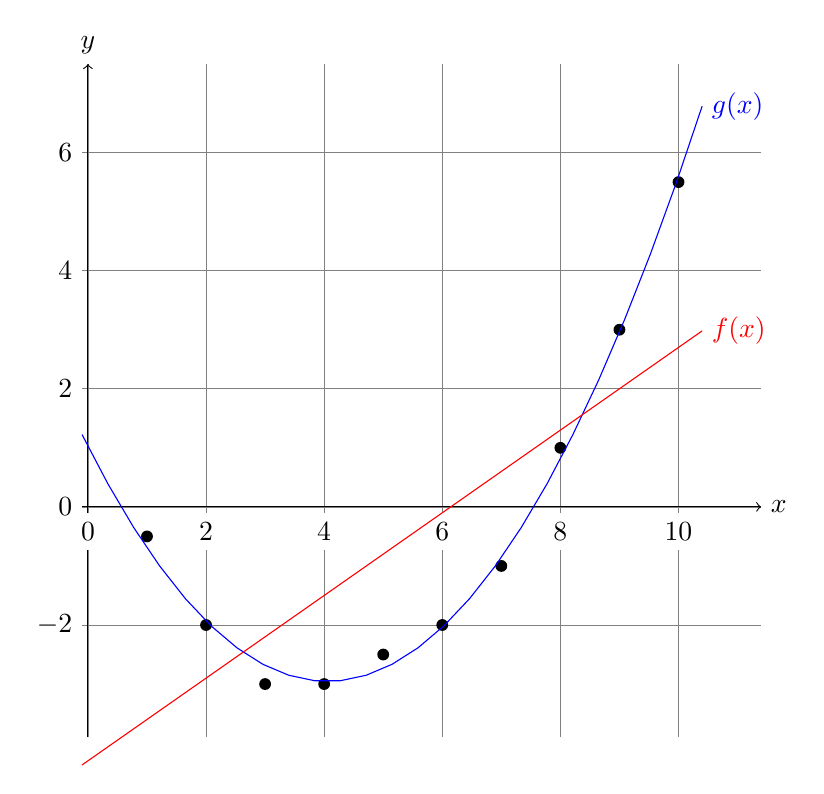
\begin{tikzpicture}[domain=-0.1:10.4,scale=0.75]
  \draw[very thin,color=gray,step=2] (-0.1,-3.9) grid (11.4,7.5);
  \draw[->] (-0.1,0) -- (11.4,0) node[right] {$x$};
  \draw[->] (0,-3.9) -- (0,7.5) node[above] {$y$};
  %\draw (-0.1,0.2) node [below left,fill=white] {0};
  \foreach \x in {0,2,4,...,10}
    \draw (\x,-0.1) node[below,fill=white] {$\x$};
  \foreach \y in {-2,0,2,4,6}
    \draw (-0.1,\y) node[left] {$\y$};
  \foreach \x/\y in
    {1/-0.5, 2/-2, 3/-3, 4/-3, 5/-2.5, 6/-2, 7/-1, 8/1, 9/3, 10/5.5}
    \fill (\x,\y) circle(0.1);
  \draw[color=blue] plot (\x,{0.242*(\x-4.056)^2-2.955}) node[right] {$g(x)$};
  \draw[color=red] plot (\x,{0.7*\x-4.3}) node[right] {$f(x)$};
\end{tikzpicture}
%\caption{$f(x) = 0.7 x - 4.3
%  \text{ und } g(x) = 0.242 (x - 4.056)^2 - 2.955$}
\caption{Regression}
\end{figure}


\begin{testproblem}
L�se folgendes, einfaches, 2-dimensionales Problem.
\begin{align}
  \min_{x \in \R^2}\ (x_1 - 1)^2 + (x_2 &- 2.5)^2 \\
  \nb -x_1 + 2x_2 & \leq 2 \\
       x_1 + 2x_2 & \leq 6 \\
       x_1 - 2x_2 & \leq 6 \\
                0 & \leq x_1, x_2
\end{align}
\end{testproblem}

\begin{figure}[ht]
\centering
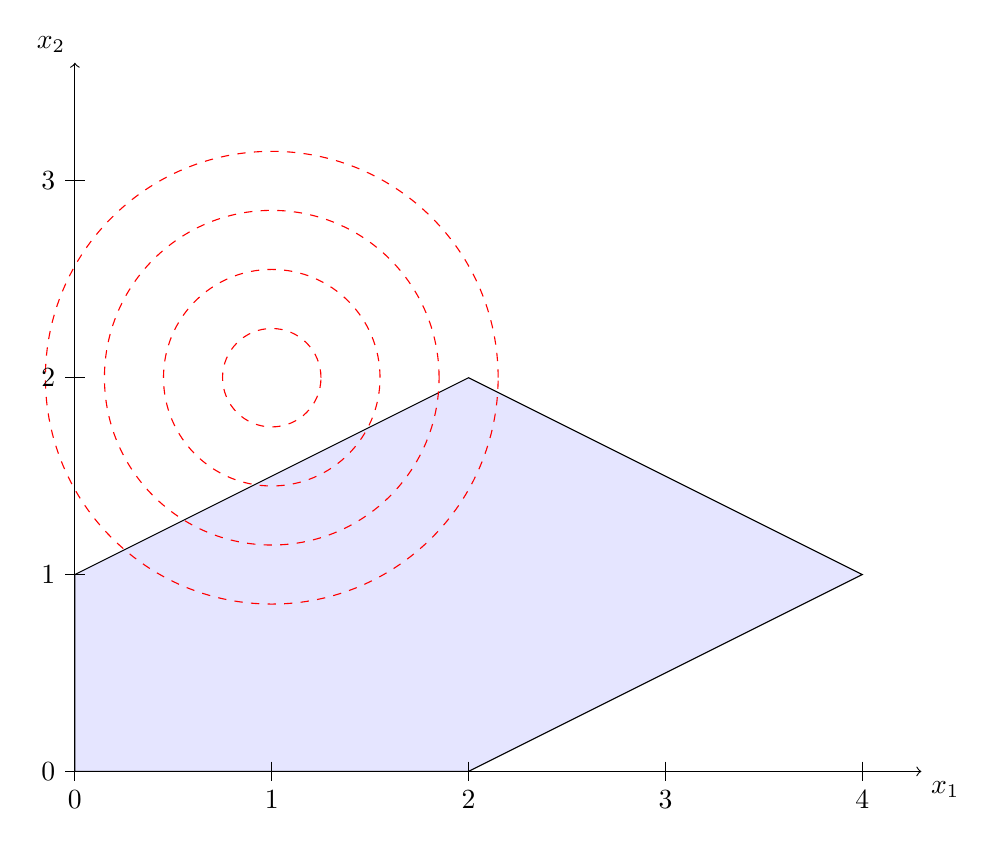
\begin{tikzpicture}[scale=2.5]
  
  % Die zul�ssige Menge
  \draw[fill=blue!10] (0,0) -- (0,1) -- (2,2) -- (4,1) -- (2,0) -- cycle;
  \draw (1.7,1) node {$\F$};
  
  % Die Niveaulinien
  \foreach \r in {0.25, 0.55, 0.85, 1.15}
    \draw[dashed,color=red] (1,2) circle (\r);
  
  % Koordinatenachsen
  \draw[->] (0,0) -- (4.3,0) node [below right] {$x_1$};
  \foreach \x in {0,...,4}
    \draw (\x,0.05) -- (\x,-0.05) node [below] {\x};
  \draw[->] (0,0) -- (0,3.6) node [above left] {$x_2$};
  \foreach \y in {0,...,3}
    \draw (0.05,\y) -- (-0.05,\y) node [left] {\y};
  
\end{tikzpicture}
\caption{Restringiertes Problem}
\end{figure}


